\documentclass{turabian-researchpaper}

\usepackage{csquotes, ellipsis}
% \documentclass[a4paper,10pt]{article}
% \usepackage[english]{babel}
% %Includes "References" in the table of contents
% \usepackage[nottoc]{tocbibind}

% Specify paper size with geometry package
\usepackage[pass, letterpaper]{geometry}
\usepackage{fancyhdr}
\usepackage{amsmath}
\usepackage{graphicx}% 用它在报告里加图
\usepackage{color}
\usepackage{enumerate}
\usepackage{amssymb}
\usepackage{siunitx}%封面表格
\usepackage{indentfirst}%第一段的首行缩进
\usepackage{pgfplots}% 使用pgfplots绘图工具包
\usepackage{graphicx} %插入图片的宏包
\usepackage{float} %设置图片浮动位置的宏包
\usepackage{subfigure} %插入多图时用子图显示的宏包
\usepackage{mathtools}
\usepackage{mhchem}
\usepackage{tensor}
\usepackage[linesnumbered, ruled]{algorithm2e}
\usepackage{braket}

\title{2000-Nodes Optimization: From Ising Model to MAX-CUT Problem by Employed Simulated Annealing and a Brief View of Quantum Annealing}
\subtitle{A Summer Research Report}
\author{Duan Jiheng}
\date{\today}

\begin{document}

\maketitle

\section{Introduction of Our Project}
    Simulated annealing(SA) is a powerful heuristic algorithm that has been formulated and applied to solve various optimization problems by a large number of people in the last forty years since Kirkpatrick published the paper \textit{Optimization by Simulated Annealing} on \textit{science} in 1983. In this article, we briefly talked about and explained what SA is including the origen, properties, relation with statistical mechanics, the controlled parameters, an example problem of applying SA: 2000-Nodes system(Ising model) optimization and also an advanced algorithm, generated from SA, called quantum annealing(QA). The SA part actually is the theoretical analysis and statements of why and how SA works. For the exact example part, the coherent Ising machine, we will give an introduction to the background of the CIM. The quantum annealing part, which is included in the future works section, is an introduction and review of quantum annealing and adiabatic quantum computation(AQC).

\section{Simulated Annealing}

    \subsection{-The description of Simulated Annealing-}
        Simulated annealing is a kind of "heuristic" algorithm. The "heuristic" here means "we could accurately approximate to the solution in the best cases, oppositely in the worst cases". This algorithm came from another heuristic algorithm called the Metropolis algorithm, first came up in 1953 and was named by Nicholas Metropolis. These heuristic algorithms are really powerful to solve combinatorial optimization problems and NP-complete problem\cite{cook2007overview} like traveling salesman problem(TSP) or knapsack problem(KP). The time complexities to find the solutions to these kinds of problems are really high for some normal algorithms. But heuristic algorithms could approximate the solution sufficiently and exactly which is the reason that they are often employed to solve these kinds of problems.

        The task of simulated annealing is to minimize or maximize the cost function denoted by $\mathcal{H} (\sigma)$ where $\sigma$ is the configuration of the optimized system. The pseudo-code of homogeneous and inhomogeneous simulated annealing are shown in Algorithm 1 and Algorithm 2\cite{chibante2010simulated}. 

            \begin{algorithm}
                initializing configuration: $\sigma_0$\;
                initializing parameters: $k = 0$, $\beta = \beta_0$, $L_k = L_0$, $\beta_c$\;
                $\mathcal{H} _0$ = $\mathcal{H} (\sigma_0)$\;
                \While{$\beta_k < \beta_c$}{
                    \For{$t=0, t < L_k$}{
                        Randomly change an neighbor in $\sigma$ then get $\sigma'$\;
                        Calculate: $\Delta \mathcal{H}  = \mathcal{H} (\sigma') - \mathcal{H} (\sigma)$\;
                        \If{$\Delta \mathcal{H}  < 0$ or $\exp(-\beta\Delta \mathcal{H} ) > uniform(0,1)$}{
                            $\sigma$ = $\sigma'$ \;
                            $\mathcal{H} (\sigma)$ = $\mathcal{H} (\sigma) + \mathcal{H} (\sigma')$ \;                   
                        }
                        t = t + 1
                    }
                    k = k + 1\;
                    Calculate: $L_{k+1}$, $\beta_{k+1}$\;
                }
                \caption{Homogeneous Simulated Annealing\cite{chibante2010simulated}}
                return($H(\sigma)$)
            \end{algorithm}
            
            \begin{algorithm}
                initializing configuration: $\sigma_0$\;
                initializing parameters: $k = 0$, $\beta = \beta_0$, $L$, $\beta_c$\;
                $\mathcal{H} _0$ = $\mathcal{H} (\sigma_0)$\;
                \While{$\beta_k < \beta_c$ and $k < L$}{
                    Randomly change an neighbor in $\sigma$ then get $\sigma'$\;
                    Calculate: $\Delta \mathcal{H}  = \mathcal{H} (\sigma') - \mathcal{H} (\sigma)$\;
                    \If{$\Delta \mathcal{H}  < 0$ or $\exp(-\beta\Delta \mathcal{H} ) > uniform(0,1)$}{
                        $\sigma$ = $\sigma'$ \;
                        $\mathcal{H} (\sigma)$ = $\mathcal{H} (\sigma) + \mathcal{H} (\sigma')$ \;                   
                    }
                    k = k + 1\;
                    Calculate: $\beta_{k+1}$\;
                }
                return($H(\sigma)$)

                \caption{Inhomogeneous Simulated Annealing\cite{chibante2010simulated}}
            \end{algorithm}

        Here $k$ is the iteration steps to count the global operation steps. $\beta$ here is thermodynamical beta defined by thermodynamical temperature $D$ and Boltzmann constant $k_B$.
            \begin{equation}
                \beta = \frac{1}{k_B D}
            \end{equation}
        And the initial temperature, $\beta_0$, is a parameter should be determined basing on different problem. In this report, we will use beta to represent the temperature. $\beta_c$ denotes the critical temperature which the system stop evolution at this temperature, so called "freezing"\cite{chibante2010simulated}. That indicates we will stop the iteration when temperature reaches $\beta_c$. For the value that initial temperature takes, many methods have been proposed in the literature to compute the initial temperature $\beta_0$\cite{ben2004computing}. It is suggested in Kirkpatrick\cite{kirkpatrick1983optimization} to take $\beta_0 = \frac{1}{k_B \Delta E_{max}}$ where $\Delta E_{max}$ is the maximal cost function difference between any two neighboring configurations. Another method is provided by Johnson which used the formula $\beta_0 = -\frac{\ln(\chi_0)}{k_B\bar{\Delta E}}$, where $\bar{\Delta E}$ is an estimation of the increase of cost function of strictly positive transitions\cite{johnson1989optimization,johnson1991optimization}. $L_k$ here means the length of a homogeneous Markov chain at temperature $\beta$ which means, see Algorithm 1 line 5, the maximum of Monte Carlo steps under a fixed temperature $\beta_k$. The difference of being described by homogeneous and inhomogeneous Markov chain between Algorithm 1 and 2 will be discussed later. From these two algorithms, the main idea of SA is to change the configuration to its neighborhood and calculate the change of the cost function. If $\Delta \mathcal{H}  < 0$, then we accept this change. But it allows the cost function goes up with some probability given by the Boltzmann factor. This criterion is called the "Metropolis criterion"\cite{chibante2010simulated}. When the temperature is high, it allows the system to jump amount most of the configurations which could forbid the cost function trapped by some local minimum valley. As the temperature lowing, the probability that the cost function reaches a higher state is small that the cost function will gradually approximate to the solution.

    \subsection{-Mechanism: Monte Carlo Steps and Markov Chain-}
        Monte Carlo steps represent a random process which, in this algorithm, is generating a random number to represent a random neighborhood(line 6 in Algorithm 1 and line 5 in Algorithm 2). The Markov chains, inside the two algorithms, are called homogeneous and inhomogeneous Markov chains. If we consider a conditional probability $P_{ij}(k|k-1)$ represents the transition probability of $(k-1)$th iteration is state i and $k$th iteration is state j. We call a Markov chain is homogeneous if this conditional probability inside it is invariant for arbitrary $k$. otherwise, we call it inhomogeneous\cite{chibante2010simulated}. An algorithm described by homogeneous Markov chains is called homogeneous algorithm(see Algorithm 1). The inhomogeneous algorithm is described by an inhomogeneous Markov chain with a temperature decreasing between each iteration(see Algorithm 2). In Algorithm 1, a single Markov chain with length $L_k$ describes a series of transitions between each configuration under a constant temperature. The temperature decreases between each Markov chain. But in Algorithm 2, the temperature decreases between each transition on a single inhomogeneous Markov chain\cite{chibante2010simulated}.

    \subsection{-The Metropolis criterion-}
        The Metropolis criterion is described by the Boltzmann factor between two configurations or, as we said in the last subsection, states with each probability denoted by $p_i$ and $p_j$ under a fixed temperature $\beta$. The probability that the system will jump from state $i$ to state $j$ is constructed by
            \begin{equation}
                \frac{p_j}{p_i} = \exp\left[-\beta(\mathcal{H} _j-\mathcal{H} _i)\right] = \exp(-\beta\Delta \mathcal{H} )
            \end{equation}
        The Metropolis criterion says: if $\Delta H < 0$ then we accept it otherwise the accepted probability is $\exp(-\beta \Delta \mathcal{H} )$. In classical computers, to employed this probability is given by a random number generator. In Algorithm 1 or 2, the implementation of this thermal jump is given by a random choice a double number in $[0,1]$. That is equivalent to the system has probability $\exp(-\beta \Delta \mathcal{H} )$ to jump to the next state. Moreover, for $\Delta \mathcal{H}  < 0$, this Boltzmann factor should always be greater than one. 

    \subsection{-Relation with Statistical Mechanics-}
        In statistical mechanics, if the average behavior is taken over the ensemble in identical systems introduced by Gibbs, where the average behavior can be characterized by an average thermal fluctuation. If so, each configuration in this ensemble of the system, described by a position sets $\{r_i\}$, is weighted by its Boltzmann probability factor $\exp\left[ \frac{-H\{r_i\}}{k_BD} \right]$ where $\mathcal{H} \{ r_i\}$ is the energy of this configuration, $k_B$ is the Boltzmann constant and $D$ is the temperature\cite{kirkpatrick1983optimization}.

        The reason why we introduced temperature into our annealing is because if $k_BT$ is smaller than $J_i$, the interaction weight between each element or the weight of each element(depends on different problems and situations), this Boltzmann factor is seen to drastically increase the efficiency of such a ground state search\cite{kirkpatrick1983optimization}.

        But in some real systems, do not contain such a temperature variable which means we could not directly analog our thermodynamic system to them. So, we introduction another controlled variable called \textit{effective temperature} to instead of thermal temperature\cite{kirkpatrick1983optimization} or just using temperature scaling factor $\beta$. This effective temperature plays the same role sd thermal temperature which is to anneal from high temperature to lower temperature.

    \subsection{-Annealing Schedules-}
        Annealing schedule is an important controlled parameter of SA which determines its cooling rate, initial temperature, "freezing" time and accuracy of the result approximation. The annealing schedule is the way that the system temperature changes. Typically, geometry annealing schedule is the most popular one which is defined by\cite{hajek1988cooling} 
            \begin{equation}
                D_t = \alpha D_{t-1}
            \end{equation}
            \begin{equation}
                D_t = \alpha^{t}D_0
            \end{equation}
        Where $t$ is the iteration steps, $D_0$ is the initial temperature and $\alpha$ is the cooling rate in range $ 0 < \alpha < 1$. Two determined parameters of this annealing schedule are $D_0$ and $\alpha$. Let's consider one example, a phase-changed solid material anneals from high temperature phase(liquid) to low temperature phase(solid). If the annealing rate is over fast, the final configuration may not drop in the ground state. That's the reason why some annealing process runs sufficiently slow. 

\section{2000-Nodes Optimization Problem}

    \subsection{-Background: Degenerate Optical Parametric Oscillator and Coherent Ising Machine-}
        In this section, we will discuss an example of using simulated annealing to deal with a combinatorial optimization problem-MAX-CUT problem of a 2000-node $K_{2000}$ graph published by \textit{Takahiro Inagaki} and \textit{Yoshitaka Haribara} in 2016. They brought out a new way to calculate the combinatorial optimization problem which is mainly known to be nondeterministic polynomial time(NP)- hard or NP complete problems. A coherent Ising machine(CIM) is one such artificial Ising machine in which a laser or a degenerate optical parametric oscillator(DOPO) represents an artificial spin inside a circular cavity. By applying the minimum-gain principle, the CIM could solve the Ising problem which we will introduce bellow.
    \subsection{-Background: Ising Model-}
        Ising model is a classical mathematical model for ferromagnetism in statistical physics which was named by Ernst Ising and Wilhelm Lenz. This model came up with analyzing and understanding the ferromagnetism of some materials, in which it consists of discrete variables that represent magnetic dipole moments of atom "spins" that can be in one of two states$(+1 \text{or} -1)$. A general Ising system is described by a Hamiltonian with the following form.
            \begin{equation}
                \mathcal{H} (\sigma) = -\sum_{<i,j>} J_{ij}\sigma_i\sigma_j - \mu\sum_j h_j\sigma_j 
            \end{equation}
            \begin{equation}
                \mathcal{H} (\sigma) = -\sum_{<i,j>} J_{ij}\sigma_i\sigma_j
            \end{equation}
        Where $\sigma_i$ means the spin state of $i^{th}$ particle, called spin configuration, takes value $\sigma \in \{1,-1\}$, $J_ij $ represents the interaction between particle $i$ and $j$, and the second term represents the effects given by an external field like a stationary magnetic field. There are various methods to analytically solve this Hamiltonian which could clearly demonstrate the ferromagnetism of this theoretical model: to set up and understand the ferromagnetic phenomenon.
        
        For a special case that this Ising Hamiltonian only exists the interaction term, which means there does not have any contribution from the external field, shown in equation (6). Then the question becomes a combinatorial optimization problem which is analog to a MAX-CUT problem, belonging to graph theory problems.
    \subsection{-Background: MAX-CUT Problem-}
        MAX-CUT problem is a typical graph theory problem that aims to find out the best configuration that minimizes the cut value $C(\sigma)$, which is defined by the sum of weight of all of the edges between each pair of vertexes respectively coming from two different sets. The configurations, denoted by $\sigma$, could represent, i.e., the spin configurations of a spin system just equivalent to the Ising model without any external field and the cost function is actually the Ising Hamiltonian. More precisely, for a $n$-particles with spin $\sigma = \{+1,-1\}$ Ising system, we separate these $n$ particles into two set $S_1 = \{\sigma = +1\}$ and $S_2 = \{\sigma = -1\}$ by their spin configurations. The cut value here becomes
            \begin{equation}
                C(\sigma) \equiv -\sum_{i\in S_1,j\in S_2}J_{ij}
            \end{equation}
        The time complexity of solving these kinds of problems, optimizing configuration $\sigma$, is NP-hard which means there is not such efficient algorithm or no polynomial-time algorithm to deal with it\cite{2016incoherent}. That is horrible for the computation.

        Therefore, the power of heuristic algorithm is stressed, which can solve these kinds of questions heuristically. Here we could using simulated annealing to solve the Ising model without an external field as an example to show how powerful the heuristic algorithm is in MAX-CUT problem. The cut value $C(\sigma)$ can be written as
            \begin{equation}
                \begin{aligned}
                    C(\sigma) &= -\sum_{i\in S_1, j\in S_2} J_{ij}\\
                    &= -\sum_{i<j} J_{ij}\frac{(1-\sigma_i\sigma_j)}{2}\\
                    &= \frac{1}{2}[-\sum_{i<j} J_{ij} - \mathcal{H} (\sigma)]
                    &= \frac{1}{2}[\sum_{ij}w_{ij}-\mathcal{H} (\sigma)]
                \end{aligned}
            \end{equation}
        Where we use $w_{ij}$ called \textit{weight} between particle $i$ and $j$ to replace the interaction amplitude $-J_{ij}$. So, the MAX-CUT problem can be transferred into a physical model and we could find out the maximum cut value as we minimize the Hamiltonian of a corresponding Ising system. The question now turns to a combinatorial optimization question which we have introduced before. Therefore, the simulated annealing works, and the results were following. \textit{Takahiro Inagaki's} team used the coherent Ising machine to solve a complete graph called $K_{2000}$ which means each two of these 2000 nodes always have edges. 
            \begin{figure}
                \centering
                \subfigure[]{
                    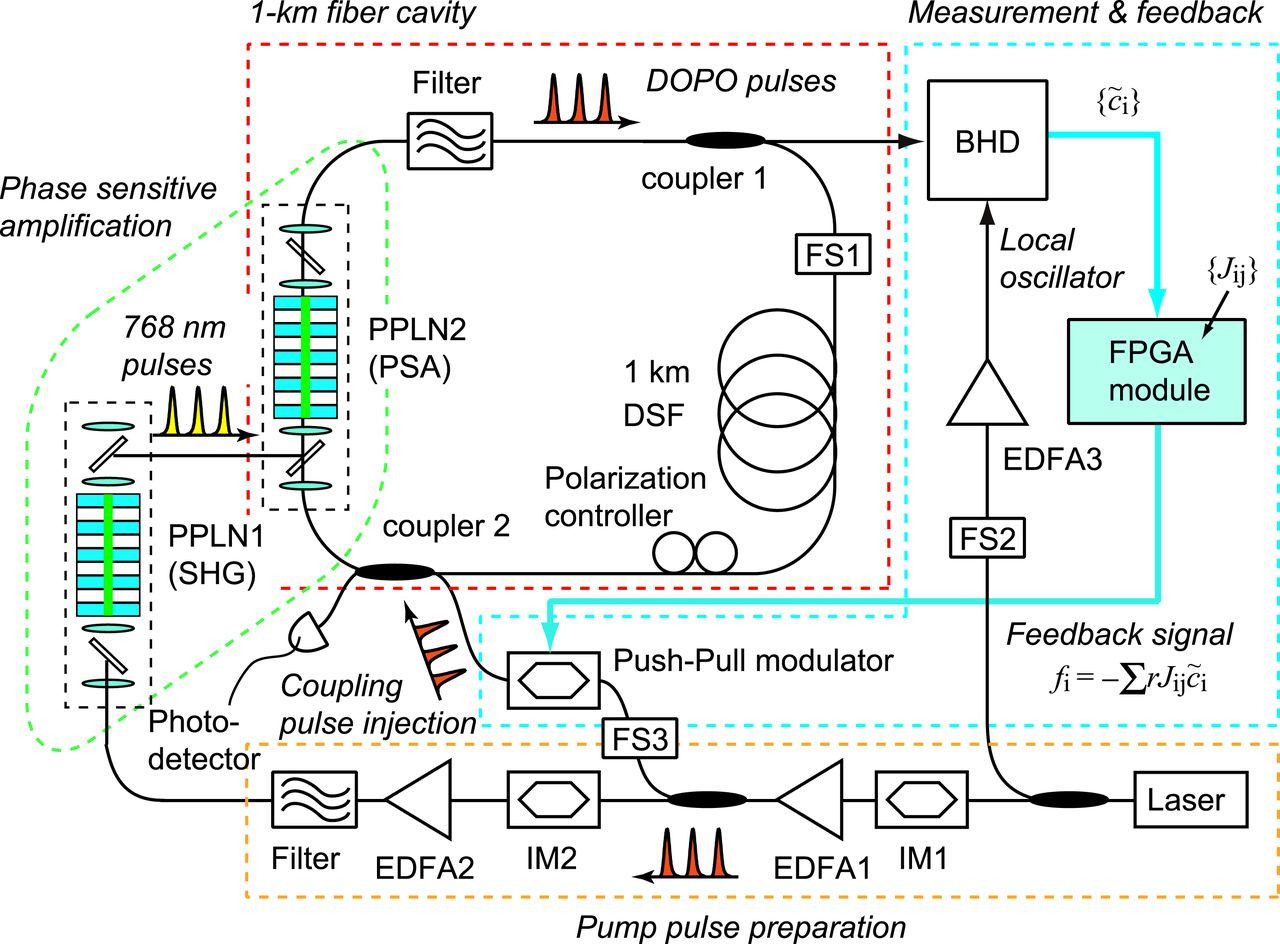
\includegraphics[width=0.5\textwidth]{Figures/F1.large.jpg}
                }
                \subfigure[]{
                    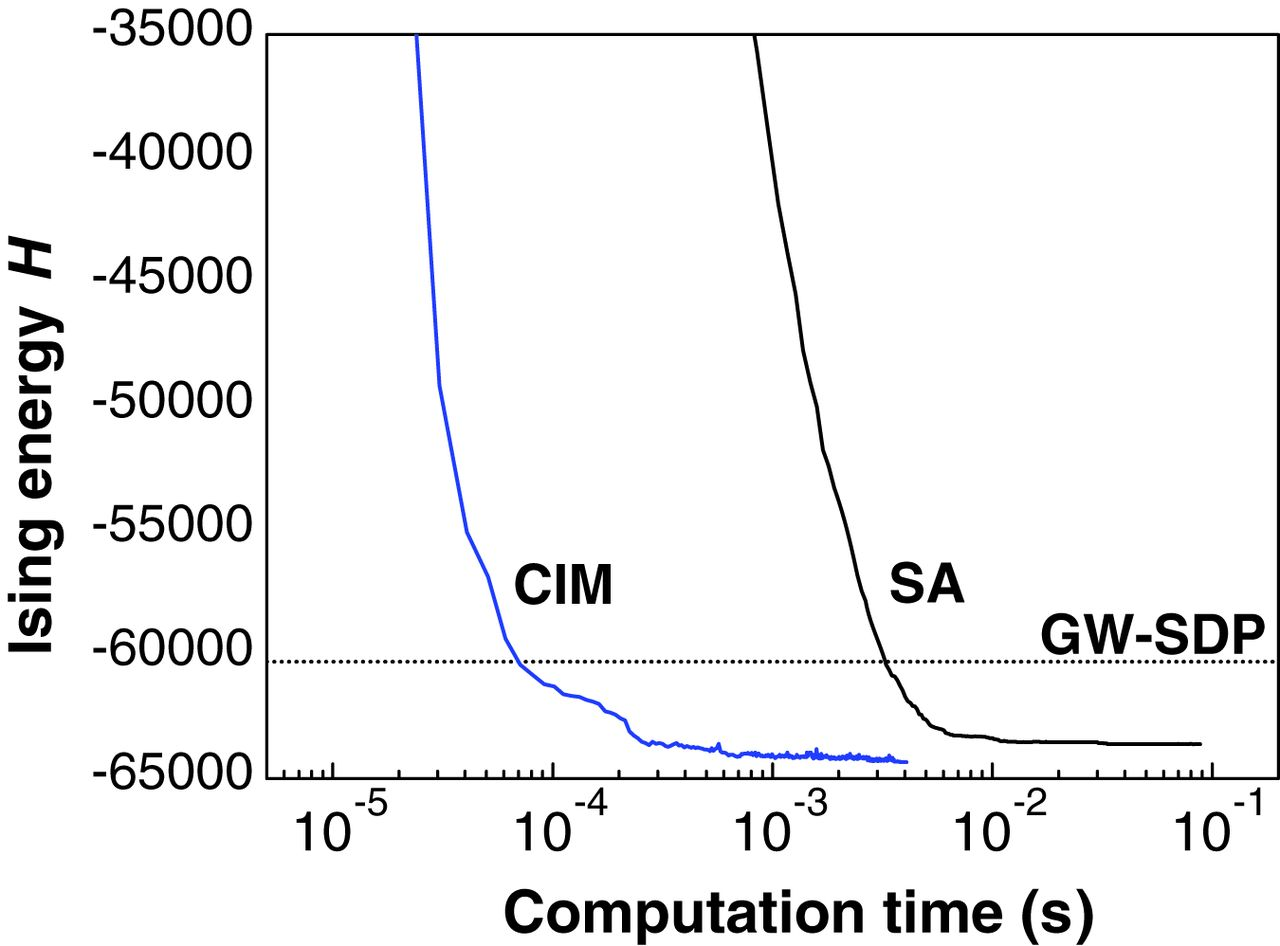
\includegraphics[width=0.4\textwidth]{Figures/F4.large.jpg}
                }
                \subfigure[]{
                    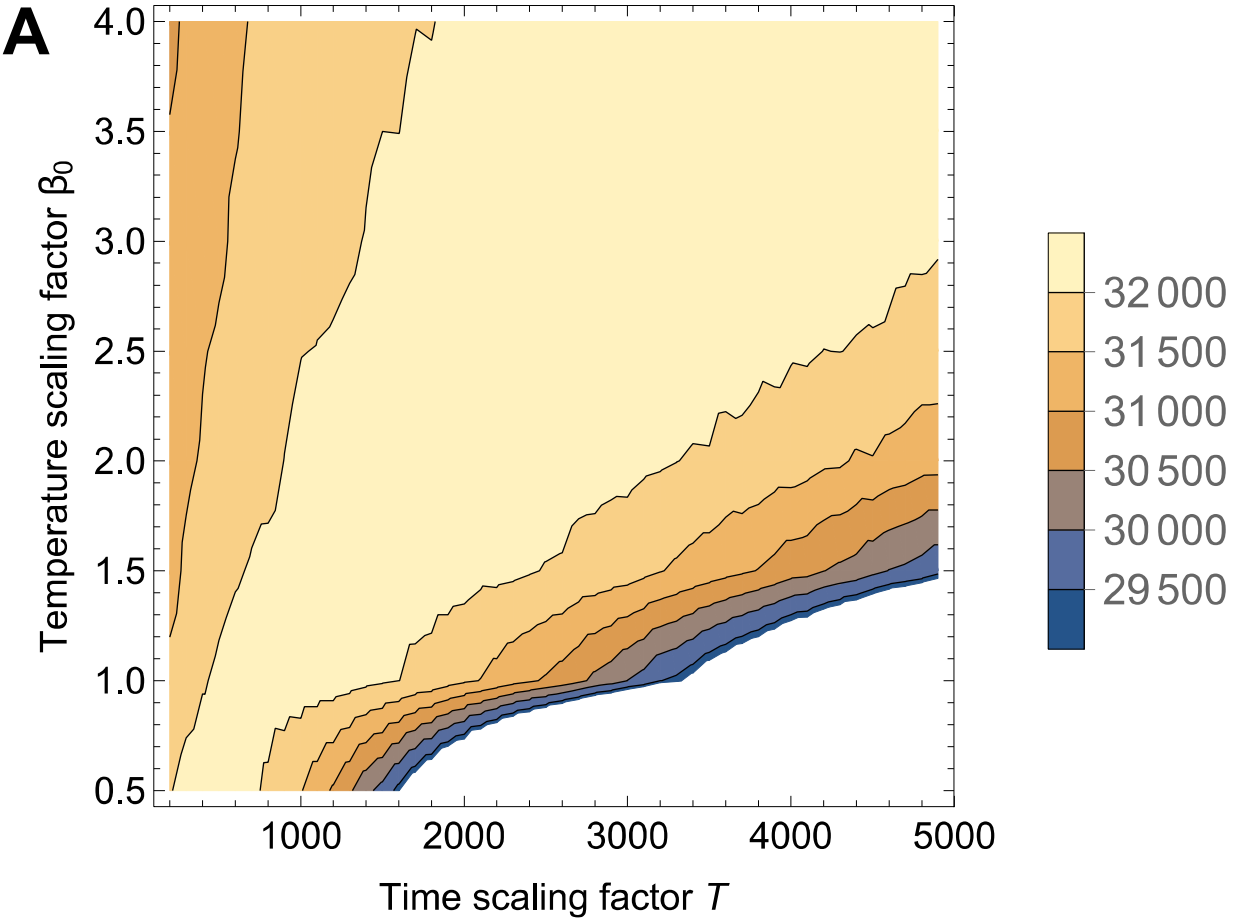
\includegraphics[width=0.4\textwidth]{Figures/F5A.png}
                }
                \subfigure[]{
                    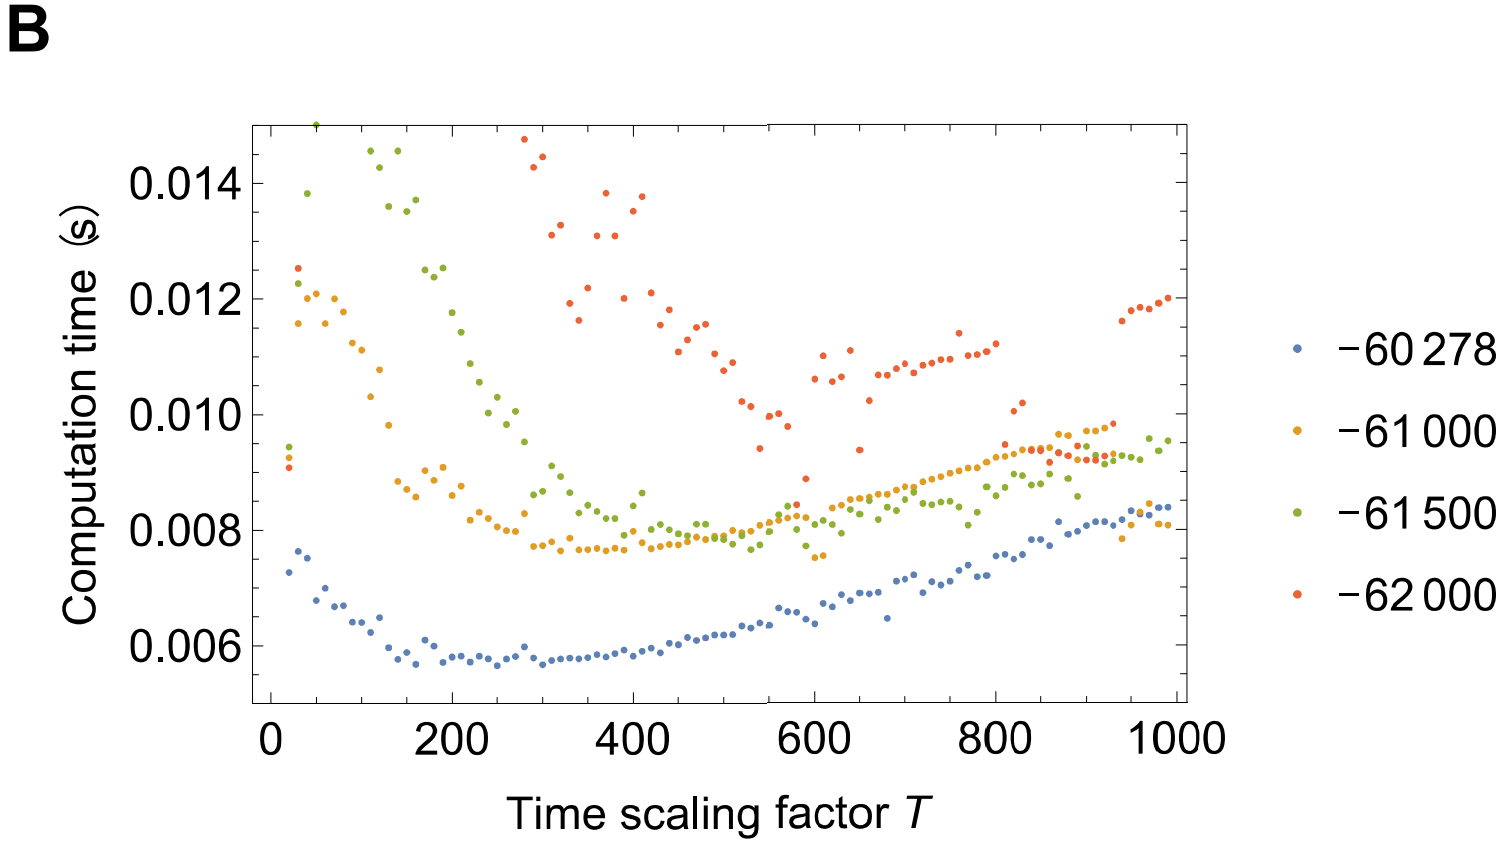
\includegraphics[width=0.5\textwidth]{Figures/F5B.png}
                }
                \caption{(a)The demonstration of coherent Ising machine with a 1-km fiber cavity\cite{2016incoherent}. (b)The computation result of graph $K_{2000}$ for the coherent Ising machine, simulated annealing, and GW algorithm. The Ising energy axis represents different cut value and the time axis means the computation time for the corresponding cut value\cite{2016incoherent}. (c)The final cut value for different time scaling factor and temperature scaling factor with 50ms fixed computation time\cite{2016incoherent}. (d)The computation time curve respects to time scaling factor for different targets energy which is the final Hamiltonian of this system\cite{2016incoherent}.}
            \end{figure}
        From Figure 1(b), we cloud find out the computation time of CIM is $10^{2}$ faster than SA and much more faster than GW algorithm\cite{2016incoherent}. The time temperature scaling factor $T$ and temperature scaling factor $\beta$ comes from the simulated annealing program written by \textit{Yoshitaka Haribara} that is shown in Algorithm 3, representing the upper bound of the annealing steps and the temperature of the system. Especially, $\beta$ here is not thermodynamical beta but proportional to $D^{-1}$ where $D$ is effective temperature. The graph adjacency matrix carrying all the information of each vertex including the weight of edges and the spin variable $\sigma$ is randomly generated as a $2000\times 1$ array. For the efficient calculation, \textit{Haribara} used a single instruction multiple data (SIMD) operation to boost an energy difference ($\Delta E$) calculation\cite{2016incoherent}. The annealing schedule was based on a logarithmic function constructed as
            \begin{equation}
                \beta = \beta_0 \log(1+t/T)
            \end{equation}
            \begin{equation}
                D = 137.6 \cdot 0.6841^t
            \end{equation}
        This schedule is different from our previous interpretation, the geometric annealing schedule, but they did the same works. The results of using a geometric annealing schedule to fit the logarithmic schedule are shown in equation (10) and Figure 2 (a). Both schedules decreased rapidly in a short period of time and then become slow and converged to zero. The \textit{Haribara's} program is uploaded to his Github with link (\text{https://github.com/hariby/SA-complete-graph}).

        \begin{algorithm}
            \SetKwFor{Loop}{loop}{}{endloop}
            Read graph adjacency matrix $J$\;
            Initialize spin variable $\sigma$\;
            $E \leftarrow \mathcal{H} (\sigma)$\;
            \Loop{}{
                $\beta \leftarrow \beta_0\log(1+t/T)$\;
                Randomly choose vertex $v \in V$\;
                $\sigma' \leftarrow flip(\sigma,v)$\;
                $\Delta E \leftarrow \mathcal{H} (\sigma') - E$\;
                \If{$\Delta E <0$ or $\exp(-\beta\Delta E) \ge \text{Uniform}(0,1)$}{
                    $\sigma \leftarrow \sigma'$\;
                    $E \leftarrow E + \Delta E$\;
                }
            }
            \Return{$E,\sigma$}
            \caption{Simulated Annealing for graph $K_{2000}$}
        \end{algorithm}
        \begin{algorithm}
            Initializing parameters\;
            Randomly initializing spin array $\sigma$\;
            $E \leftarrow \mathcal{H} (\sigma)$\;
            \While{$t < T+1$}{
                $\beta \leftarrow \beta_0\log(1+t/T)$\;
                $\sigma' \leftarrow flip(\sigma,v)$\;
                $\Delta E \leftarrow \mathcal{H} (\sigma') - E$\;
                \If{$\Delta E <0$ or $\exp(-\beta\Delta E) \ge \text{Uniform}(0,1)$}{
                    $\sigma \leftarrow \sigma'$\;
                    $E \leftarrow E + \Delta E$\;
                    $t = t + 1$\;
                }
                \Else{
                    $t = t$
                }
            }
            \Return{$E, \sigma$}\;
            \caption{Simulated Annealing for graph $K_{2000}$ via python}
        \end{algorithm}

        % the path of a salesman traveling between a set of cities with some specific order in "Traveling Salesman's Problem"(TSP) or the tag of the items chosen to put in bags in Knapsack problems. Similarly, it can also represent
    \subsection{-Coding by Python-}
        Basing on \textit{Haribara's} pseudo code, we reconstructed a program via python to realize the simulated annealing process to solve the $K_{2000}$ complete graph MAX-CUT problem. The algorithm pseudo-code was shown in Algorithm 4. The basic structure of our pseudo code is similar to \textit{Haribara's} without else statement which controlled the steps in one homogeneous Markov chain or say our algorithm is homogeneous and the other is inhomogeneous. The calculation results are shown in Figure 2 (b) which indicated the calculation time is much slower than \textit{Haribara's}. The main reason is the calculation of energy difference $\Delta E$. Instead of using the SIMD process, we using the order property to simplify the calculation. We found that the speed of calculation for different types of algorithms is nearly the same, but the upper limit of calculation results, the Ising Hamiltonian, the homogeneous one is higher than the inhomogeneous one. The upper limit of calculation results is the maximum of cut value, as we see in Figure 2 (b), the Homogeneous SA fluctuated around $H(\sigma) = -10000$ under time scaling factor $T = 4$ and initial temperature scaling factor $\beta_0 = 4$. The python file was uploaded on Github with a link(https://github.com/RunawayFancy/SA-complete-graph).

        \begin{figure}
            \centering
            \subfigure[]{
                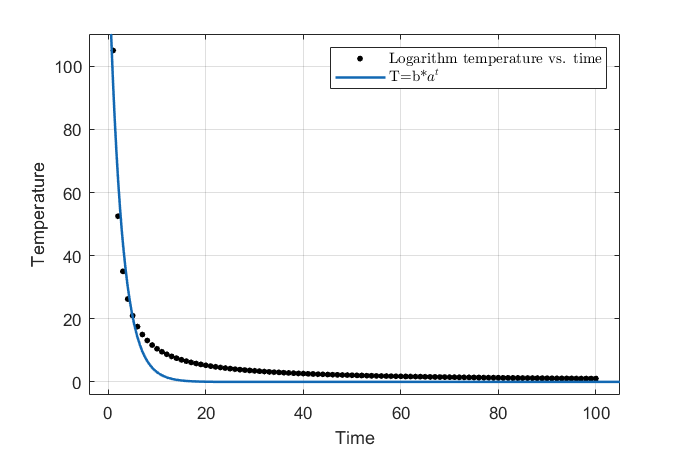
\includegraphics[width=0.45\textwidth]{Figures/Logrithm-fitting.png}
            }
            \subfigure[]{
                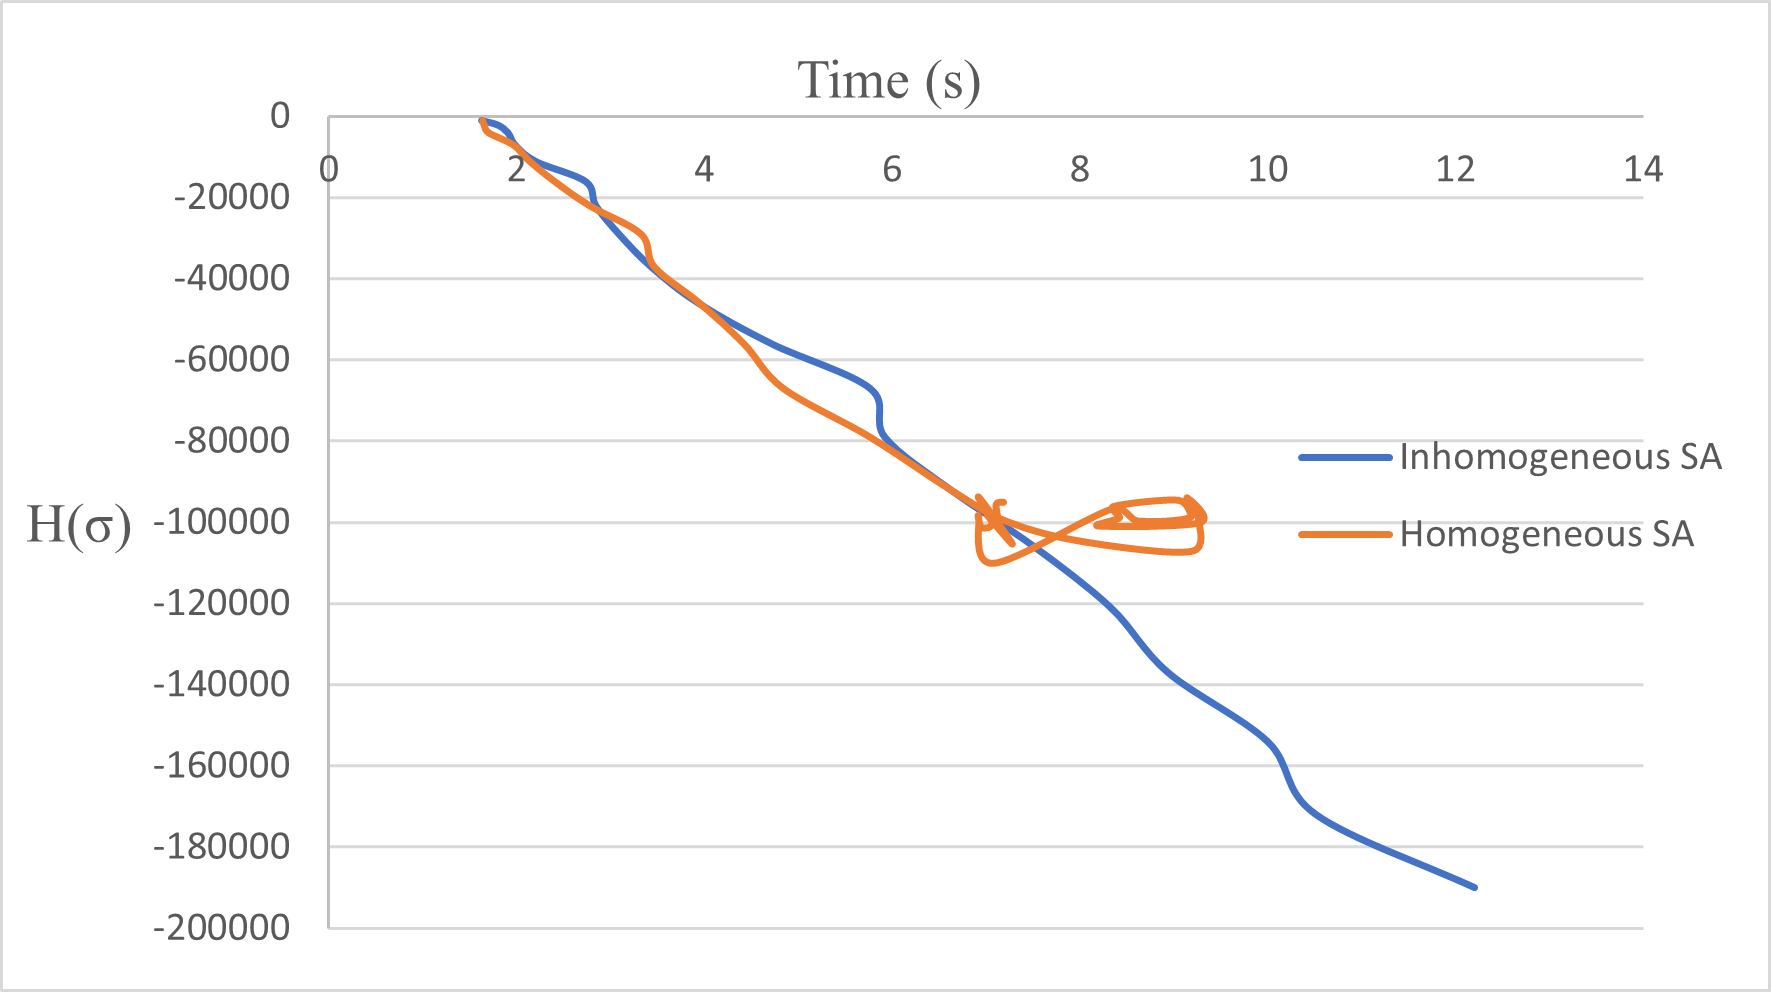
\includegraphics[width=0.45\textwidth]{Figures/Figure2-homo vs inhomo.png}
            }
            \caption{(a)Basing on the logarithm annealing schedule, we plot out the temperature-time figure and using a geometric annealing schedule to fit it. The result shows that the changes of ratio and tendency both are perfectly the same which indicates the rationality of using a logarithm annealing schedule. (b)The comparison of computational abilities between homogeneous and inhomogeneous simulated annealing algorithms. For the situation that time scaling factor $T = 4200$ and initial temperature scaling factor $\beta_0 = 4$, the upper limit of the computation ability, the Hamiltonian(cut number), for homogeneous SA is lower than inhomogeneous SA.}
        \end{figure}
\section{A Brief View of Quantum Annealing}
    Quantum annealing(QA) is a pure physical algorithm based on quantum adiabatic theorem and classical annealing theory describes a quantum fluctuation between different states of some particle in spin glass. As it came from classical simulated annealing, quantum annealing was also an annealing process from high "temperature" states to low "temperature" states but am adiabatic process. The "temperature" here is not thermodynamical temperature but a representation of the amplitude of the driving field $\Gamma$ which contributes to a quantum fluctuation. With the fluctuation, based on quantum tunneling, the system's configuration could come over the potential barrier and reach the lower energy state. The quantum adiabatic theorem, which was theoretically proofed by \textit{Tosio KATO} in 1950, generally for a Hamiltonian $H$ controlled by some parameters, interpret that if the parameters change on time scale $T$ that is much larger than $\frac{2\pi}{\omega_{ab}} = \frac{2\pi\hbar}{E_{ab}}$ for some difference $E_{ab}$ in energy eigenvalues, then the energy eigenvalues should just follow the values one gets as the parameters themselves change. So that indicates if the system Hamiltonian evolutes from high  $\mathcal{H} (0)$ to a stable value $\mathcal{H} (t)$ and the system stays in the ground state $\ket{0}$, then it will remain in ground state after the evolution of system Hamiltonian. That is the reason why we could use quantum annealing to find a system's ground state. If we assume the spin state of a single particle denoted by $\sigma$ and $J_{ij}$ denotes the coupling strength between two particles. By Suzuki-Trotter formalism, the Hamiltonian of the annealing system is shown in equation (11). Here $\Gamma$ is a time-decreasing driving field that reduces to zero slowly after a period of time which indicates the quantum fluctuation is strong at the start time and reduces to zero in the end as the system cools down. This formalism is similar to the quantum adiabatic computation, see equation (12) where parameter $s$ vary slowly from $0$ to $1$. $\mathcal{H} _0$ and $\mathcal{H} _F$ represent initial and target Hamiltonian for this process. In 2011, \textit{M. W. Johnson, M. H. S. Amin} and other people published the paper \textit{Quantum annealing with manufactured spins}\cite{johnson2011quantum} focusing on using quantum annealing to calculate the ground state of eight flux qubits, technic of how to design a sample and method they controlled the system. They also talked about the contribution given by thermodynamical fluctuation and quantum fluctuation and under what situations that each of them affected jumping to the lower energy state. \textit{M. W. Johnson and M. H. S. Amin's } team using two-level system shows when temperature above 45mK, the upper energy level in the flux qubits start to become thermal occupied and four-level quantum model describes the behavior of the system well up to 80mK, where more energy level starts to be occupied\cite{johnson2011quantum}. 
    \begin{equation}
        \mathcal{H}  = -\Gamma \sum_{i=1}^{N} \sigma_i^x - \sum_{<i,j>} J_{ij} \sigma_i^z \sigma_j^z
    \end{equation}
    \begin{equation}
        \mathcal{H}  = (1-s) \mathcal{H} _0 + s \mathcal{H} _F, \ \ s\in [0,1]
    \end{equation}
    \begin{figure}
        \centering
        \subfigure[]{
            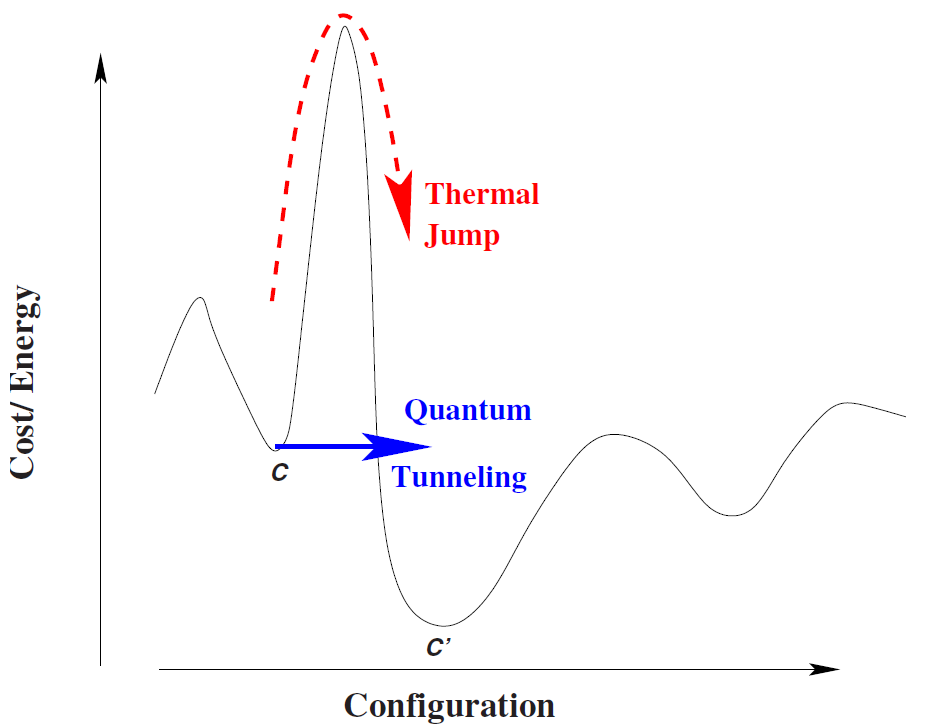
\includegraphics[width=0.45\textwidth]{Figures/QA-ComparingWithThermalJump.png}
        }
        \subfigure[]{
            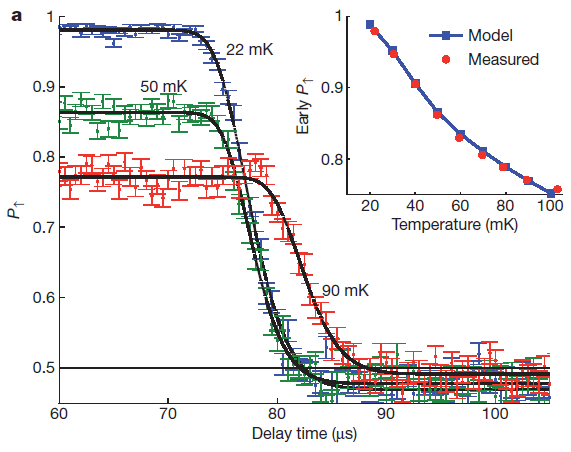
\includegraphics[width=0.45\textwidth]{Figures/flux-qubits-annealing-1.png}
        }
        \subfigure[]{
            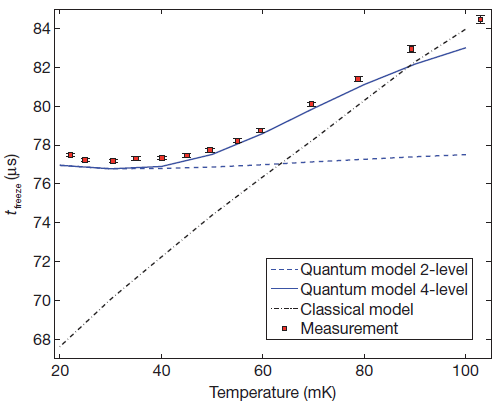
\includegraphics[width=0.45\textwidth]{Figures/flux-qubits-annealing-2.png}
        }
        \subfigure[]{
            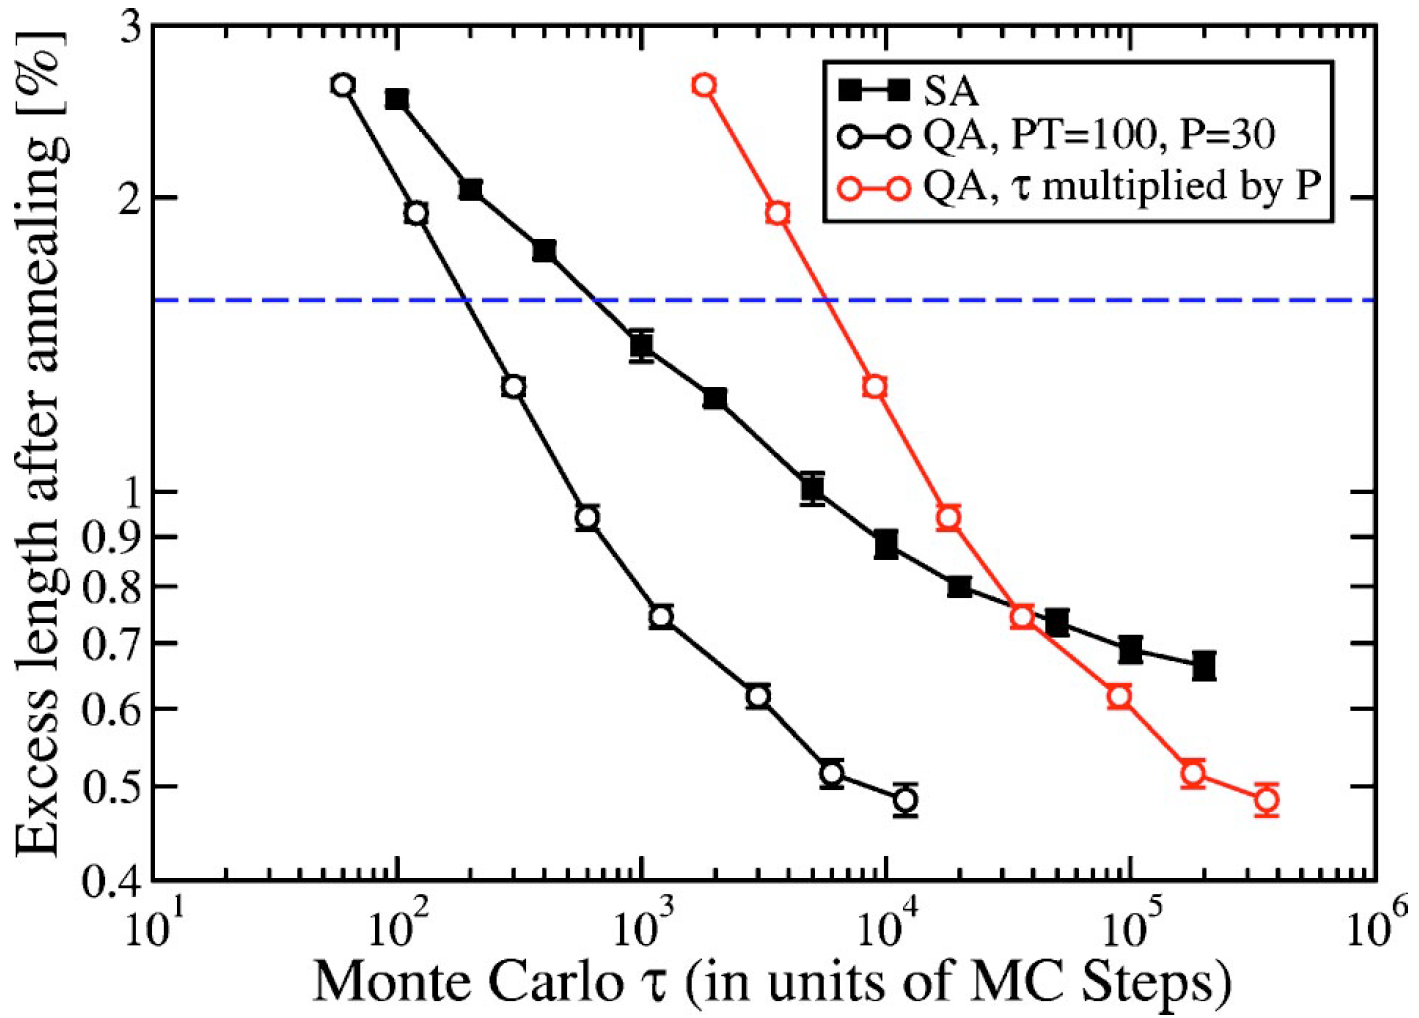
\includegraphics[width=0.45\textwidth]{Figures/Quantu-MonteCarlo-TSP.png}
        }
        \caption{(a)Picture of the difference between thermal jump and quantum tunneling in go through the energy barrier to achieve the global minima instead of being trapped by local minima\cite{das2008colloquium}. (b)A measurement of final ground-state probability, $P_{\uparrow}$, in single qubit versus the delay time $t_d$, which is the time they increase the energy difference between ground state and excited state, of a step $h_t = 2.55\pm 0.04GHz$ in energy basis, for $T=22mK$(blue), $50mK$(blue) and $90mK$(red). the solid lines are the result of fits used to extract the freeze-out time$t_{freeze}$. Inset, measured and simulated(four-level quantum models) T dependence of $P_\uparrow$ for $t_d = 0$\cite{johnson2011quantum}. (c)For single qubit system, under different temperature, measured the freeze time versus T(red points). The simulation of two-level(dashed blue) and four-level(solid blue) quantum mechanical models and form a classical model of the qubit(black)\cite{johnson2011quantum}. (d)Using quantum Monte Carlo method to solve traveling salesman problem. It shows that average residual excess length found after Monte Carlo annealing for a total time $\tau$(in Monte Carlo steps), for the city number $N=1002$. And the results briefly shows how quantum annealing or the quantum Monte Carlo method provides provides residual excess lengths decaying faster than classical simulated annealing\cite{martovnak2004quantum}.} 
    \end{figure}

    D:WAVE company built up the world's first business used quantum computer whose core computational principle is quantum annealing. Today, people could also use Python to import the quantum annealing library to realize simulated quantum annealing, which we would talk about it later. The problem that quantum annealing could handle is just as simulated annealing: combinatorial optimization problem. But QA can put more effort into reducing the computation time complexity which means it calculates faster than classical algorithm\cite{crosson2016simulated}. As an example, we could find in \textit{Roman Martonak}'s paper \textit{Quantum annealing of the traveling-salesman problem}\cite{martovnak2004quantum}, the computational speed of simulated quantum annealing is obviously faster than simulated annealing, see Figure 3(b)\cite{martovnak2004quantum}. Notice that instead of directly using quantum annealing, they reform the Hamiltonian into a transverse Ising form\cite{elliott1970ising} and used simulated a quantum annealing method called quantum Monte Carlo which means they using Monte Carlo path integral to forbid to directly do Schrodinger annealing evolution of quantum Hamiltonian. The simulated quantum annealing is a classical algorithm that relates certain quantum systems to classical Markov chains\cite{crosson2016simulated}. By proving that these chains mix rapidly, we show that simulated quantum annealing runs in polynomial time on the problem where quantum annealing achieves an exponential advantage over SA\cite{crosson2016simulated}. The variation of the quantum Monte Carlo method was previously mentioned in connection with finding good importance functions and beginning the ensemble, as it was the adaptation of the classical Metropolis algorithm\cite{ceperley1986quantum}. The mathematical formalism of quantum Monte Carlo is shown in equation (13) where we want to find the matrix element of the partition function $Z$ between two energy eigenstates $\ket{M}$ and $\ket{N}$, as $M,N\in \mathbb{Z}$. If we define the number of states between $\ket{M}$ and $\ket{N}$ denoted by $\Delta$ is $\Delta = M-N+1$. Then, the matrix element can be transferred to equation (14) which means we only need to calculate the neighbored matrix elements and then multiple them up. This process is similar to a random walk between two states which is the concept of the classical Monte Carlo method. 
    
    \begin{equation}
        Z = \exp(-\frac{\mathcal{H} }{k_B T}) = \exp(-\beta \mathcal{H})
    \end{equation}
    \begin{equation}
        \begin{aligned}
            \braket{M|\exp(-\beta \mathcal{H} )|N} &= \braket{M|\exp(\frac{-\beta \mathcal{H}}{\Delta})|M-1}\braket{M-1|\exp(\frac{-\beta \mathcal{H}}{\Delta})|M-2} \\
            &\braket{M-2|\exp(\frac{-\beta \mathcal{H}}{\Delta})|M-3}\cdots\braket{N+1|\exp(\frac{-\beta \mathcal{H}}{\Delta})|N}\\
        \end{aligned}
    \end{equation}

\section{Conclusions}
    From the annealing process of metal to the Metropolis algorithm then, to the classical simulated annealing finally reached the quantum annealing, these kinds of heuristic algorithms came from natural phenomenon and the theory in people's mind then go through the computer's simulation finally applied in a quantum physical system. The power of these heuristic algorithms for dealing with combinatorial optimization problems was thoroughly presented. For quantum annealing, the future of this technic is bright for some businesses use like courier companies to properly arrange their staffs to serve the different areas or minimize the cost of traveling paths. The reach area that quantum annealing belongs to, the quantum adiabatic computation, has more development potential. Big companies such as Google are majoring in research in this area which provided lots of resources to develop this technic. we believe that gaining further experience with the quantum model and qubits model represents a very promising and challenging route, particularly in view of the future development of quantum adiabatic computation.
\bibliographystyle{IEEEtran}
\bibliography{citation}

\end{document}